% Created 2020-11-17 二 21:21
% Intended LaTeX compiler: xelatex
\documentclass[11pt]{report}
\usepackage{graphicx}
\usepackage{grffile}
\usepackage{longtable}
\usepackage{wrapfig}
\usepackage{rotating}
\usepackage[normalem]{ulem}
\usepackage{amsmath}
\usepackage{textcomp}
\usepackage{amssymb}
\usepackage{capt-of}
\usepackage{hyperref}
\author{曹嘉祺 PB18030874 化学与材料科学学院 有机化学系 \thanks{中国 安徽合肥 中国科学技术大学 Email: \href{mailto:mkq@mail.ustc.edu.cn}{mkq@mail.ustc.edu.cn}}}
\usepackage[scheme=plain]{ctex}
\usepackage{fontspec}
\setmainfont{更纱黑体 UI SC}
\hypersetup{colorlinks=true,linkcolor=blue}
\usepackage{longtable}
\date{\today}
\title{正丁醇偶极矩的测定}
\hypersetup{
 pdfauthor={曹嘉祺 PB18030874 化学与材料科学学院 有机化学系},
 pdftitle={正丁醇偶极矩的测定},
 pdfkeywords={},
 pdfsubject={},
 pdfcreator={Emacs 27.1 (Org mode 9.4)}, 
 pdflang={English}}
\begin{document}

\maketitle
\tableofcontents

\begin{abstract}
 本实验通过对正丁醇的环己烷溶液的折射率、介电常数和密度随浓度的变化进行
测量,利用外推法得到线性关系系数,从而求得正丁醇的固有偶极矩。通过本实验我们了解
了偶极矩测定的基本原理和基本方法,同时掌握了溶液法测定正丁醇偶极矩的实验方法。


\noindent\rule{\textwidth}{0.5pt}
\begin{itemize}
\item 关键词: 正丁醇\quad 偶极矩\quad 折射率\quad 介电常数\quad 密度\quad 外推法\quad 线性相关系数
\end{itemize}
\end{abstract}
\begin{abstract}
In this experiment, we determine the refractive indexes, dielectric constants and
density of 1-butanol \& cyclohexane solution under different concentrations. Then we determine
the linear related coefficients by using extrapolation. And finally we get the intrinsic dipole
moment of 1-butanol. During this experiment, we learned the basic principles and methods of
determining the intrinsic dipole, as well as the experimental method of detecting the intrinsic
dipole by solution.

\noindent\rule{\textwidth}{0.5pt}

\begin{itemize}
\item key words: Dipole Moment; Density;Capacity;Refractive Index
\end{itemize}
\end{abstract}
\part{前言}
\label{sec:org336eb4a}
假设一个中性分子的正负电荷中心不重合,则此分子的静电学性质可以简化为图中所示
的电偶极子模型,其中\vec{r} 是由负电中心到正电中心的向量,q 是正或负电荷电量的绝对值。
那么偶极矩
\[
\vec{\mu}= q\vec{r}
\]
分子的正负电荷中心不重合,可以是这一分子在无外界电场作用下就能表现出的固有属性
——此时它被称为“极性分子”;也可以是正负电荷中心原本重合的“非极性分子”,在外
电场作用下发生了正负电荷中心的相互分离。因此偶极矩大小定量的表现出分子当前极性程
度的大小,本实验就是要测定极性分子正丁醇的固有偶极矩大小。
\chapter{实验原理}
\label{sec:org8cd4277}
\section{偶极矩和极化度}
\label{sec:org937c065}
分子结构可以被看成是由电子和分子骨架所构成。由于其空间构型不同其正负电荷中心
可以重合,也可以不重合,前者称为非极性分子,后者称为极性分子,分子的极性可用偶极
矩来表示。两个大小相等符号相反的电荷系统的电偶极矩的定义为
\[
\vec{\mu}= q\vec{r}
\]
式中\vec{r}是两个电荷中心间距矢量,方向是从正电荷指向负电荷。
电介质分子处于电场中,电场会使非极性分子的正负电荷中心发生相对位移而变得不重
合,电场也会使极性分子的正负电荷中心间距增大这样会使分子产生附加的偶极矩(诱导偶
极矩)。这种现象称为分子的变形极化。
\section{极化度的测量}
\label{sec:org4ff51db}
如将电介质置于交变电场中,则其极化和电场变化的频率有关。
当交变电场的 频率进一步增加到大于 10\textsuperscript{15}\(\cdot\) s\textsuperscript{-1} 高频场(可见光和紫外)时,分子的取向和
分子骨架的变形都跟不上电场的变化,这时 P\textsubscript{O} = 0、P\textsubscript{A} = 0、 P = P\textsubscript{E}。这时\(\varepsilon\) = n\textsuperscript{2},
n 为介质的折射率,这时的摩尔极化度称为摩尔折射度 R:
\[
P_{E}=R=\frac{n^{2}-1}{n^{2}+2}\cdot \frac{M}{\rho}
\]
因为 P\textsubscript{A} 只有 P\textsubscript{E}的10\%左右,一般可以略去,或按 P\textsubscript{E}10\%修正。
可得:
\[
\mu=\left(\frac{9K}{4\piN_{0}}\right)^{\frac{1}{2}}\left(P-P_{E}-P_{A}\right)^{\frac{1}{2}}T^{\frac{1}{2}}
\]
略去 P\textsubscript{A}可得:
\[
\mu=\left(\frac{9K}{4\piN_{0}}\right)^{\frac{1}{2}}\left(P-R\right)^{\frac{1}{2}}T^{\frac{1}{2}}
\]
\[
\mu=0.0128\sqrt{(P-R)T}
\]
由上式计算 E\textsubscript{内}忽略了分子间相互作用项 F\textsubscript{4},故用无限稀的 P\textsuperscript{\(\infty\)}、R\textsuperscript{\(\infty\)}:
\[
\mu=0.0128\sqrt{(P^{\infty}-R^{\infty})T}
\]
所以我们在实验中要测不同浓度下的 P、R,再用外推法求 P\textsuperscript{\(\infty\)}和 R\textsuperscript{\(\infty\)}。
对于由溶剂 1 和溶剂 2 组成的溶液体系,根据 Hedestrand(Z. Phys. Cnem.,2438(1929))
的理论,其介电常数、折射率、摩尔极化度以及密度均和浓度成线性关系,即:
\[
\varepsilon =\varepsilon_{1}(1+\alpha X_{2})
\]
\[
n =n_{1}(1+\gamma X_{2})
\]
\[
\rho =\rho_{1}(1+\theta X_{2})
\]
\[
P =X_{1}P_{1}+X_{2}P_{2}
\]
式中 X\textsubscript{1}、X\textsubscript{2} 分别为溶剂和溶质的摩尔分数,\(\varepsilon\)、\(\rho\)、P、n;\(\varepsilon\)\textsubscript{1}、\(\rho\)\textsubscript{1}、P\textsubscript{1}、n\textsubscript{1};\(\varepsilon\)\textsubscript{2}、\(\rho\)\textsubscript{2}、P\textsubscript{2}、n\textsubscript{2}
分别为溶液、溶剂和溶质的介质常数、密度、摩尔极化度和折射率,\(\alpha\)、\(\beta\)、\(\gamma\) 为常数。由此
可得:
\[
P^{\infty}=P^{\infty}_{2}=\lim_{X_{2}\to 0}P_{2}=\frac{3\alpha\varepsilon_{1}}{(\varepsilon_{1}+2)^{2}}\cdot\frac{M_{1}}{\rho_{1}}+\frac{\varepsilon_{1}-1}{\varepsilon_{1}+2}\cdot\frac{M_{2}-\beta M_{1}}{\rho_{1}}
\]
\[
R^{\infty}=R^{\infty}_{2}=\lim_{X_{2}\to 0}R_{2}=\frac{n_{1}^{2}-1}{n_{1}^{2}+2}\cdot\frac{M_{2}-\beta M_{1}}{\rho_{1}}+\frac{6n_{1}^{2}M_{1}r}{(n_{1}^{2}+2)^{2}\rho_{1}}
\]
这样我们用交变频率为 1000Hz 的交流电桥测出电容池中各浓度下溶液的电容,用此电
容除以真空下电容池的电容即得介电常数。用阿贝折射仪测出可见光下各溶液的折射率,再
用分析天平测出各溶液的密度代入上面各式,可定出 \(\alpha\)、\(\beta\)、\(\gamma\),并算出 P\textsuperscript{\(\infty\)}和 R\textsuperscript{\(\infty\)}
,最后算出分子的永久偶极矩 \(\mu\)。

\part{实验部分}
\label{sec:orgb8d66d1}
\chapter{实验仪器与试剂}
\label{sec:org2a09ba0}
\section{仪器}
\label{sec:orgb25879d}
\begin{center}
\begin{tabular}{lrl}
仪器 & 数目 & 厂家\\
\hline
阿贝折射仪 & 1 & 上海实验仪器厂有限公司\\
分析天平 & 1 & \\
干燥器 & 1 & \\
电吹风 & 1 & \\
比重瓶 & 1 & \\
电容池 & 1 & \\
CCJ-1 型精密电容测量仪 & 1 & 南大应用物理研究所\\
超级恒温槽 & 1 & 上海实验仪器厂有限公司\\
容量瓶(25 ml) & 6 & \\
\end{tabular}
\end{center}

\section{试剂}
\label{sec:org7a7ac5c}
\begin{enumerate}
\item 正丁醇
\label{sec:orgf19802e}
\begin{itemize}
\item 纯度:分析纯 AR
\item 性状:无色透明液体
\item 分子量:M=74.12
\item 型号:T20100305
\item 厂家:国药集团化学试剂有限公司
\end{itemize}
\item 环己烷
\label{sec:orgc5d7acf}
\begin{itemize}
\item 纯度:分析纯 AR
\item 性状:无色透明、易燃液体
\item 分子量:M=84.16
\item 型号:T20100817
\item 厂家:国药集团化学试剂有限公司
\end{itemize}
\end{enumerate}

\chapter{实验步骤}
\label{sec:org43ec225}
\section{溶液配置}
\label{sec:org070f5c2}
    用称量法配制 0\%、1\%、5\%、10\%和 15\%(摩尔分数)的环已烷溶液各 20 毫升(除 0\%
外,其余溶液的浓度只要求精确标出浓度值,其值控制在 1\%、5\%、10\%、15\%左右)
 。操作时应注意防止溶质、溶剂的挥发以及吸收水汽。为此溶液配好后应迅速盖上瓶盖并置于干燥
器中。
\section{折射率的测定}
\label{sec:org7fc8707}
用阿贝折射仪测出溶液的折射率。测定时各样品需加样三次,每次取三个数据,最后取
平均值。
\section{介质常数的测定}
\label{sec:org5a2a94f}
\begin{enumerate}
\item 电容池分布电容C\textsubscript{d} 和真空电容 C\textsubscript{o} 的测定
\label{sec:orgd6b88dc}
因为电容池总是存在着和真空电容 C\textsubscript{o} 并联的分布电容 C\textsubscript{d},为了从实测溶液的电容中扣
除此分布电容的影响,我们必须测出此分布电容。
用电吹风将电容池二极间的空隙吹干,旋上金属盖,将恒温槽电源打开,使温度固定在
某一实验工作温度,测定其电容 C\textsubscript{o}。测量中要反复交替调节相位平衡旋钮,使表头指针趋
于最小,电桥平衡后,读出电容值,重复调节三次,以三次读数的平均值。
再用针筒吸取纯环已烷加入电容池,使液面超过二电极表面。恒温数分钟后如上述步骤
测定电容值。然后打开金属盖,用针筒吸取二极间的环已烷,重新装入样品,再次测定电容
值,取二次平均值为 C\textsubscript{环}。
\end{enumerate}
\section{加溶液电容的测定}
\label{sec:orga0f67ce}
测定方法同于纯环已烷。重复测定时,要去掉电极间的溶液,还要用电吹风将二极间的
空隙吹干,然后再加入该浓度溶液,恒温数分钟,测出电容值。两次测定数的差值应小于
0.05PF,否则要重新测量。测得的电容减去 C\textsubscript{d} 后才是该溶液对应的电容值。
\section{溶液密度的测定(改用密度仪)}
\label{sec:orgfeb3b5d}
用比重瓶在分析天平上分别称得瓶重 W\textsubscript{0},加液后的质量 W\textsubscript{1},和加水后的 W\textsubscript{2},按
\[
\rho_{溶}=\frac{W_{1}-W_{0}}{W_{2}-W_{0}}\rho_{水}(t)
\]
计算溶液的密度 \(\rho\)\textsubscript{溶}。式中 \(\rho\)\textsubscript{水}(t)为在工作温度下的密度,可由表中查出。
测量中要避免比重瓶中气泡的产生,等测完所有溶液的密度后,才加水测量 W\textsubscript{2}。
\chapter{实验数据及数据处理(见附件)}
\label{sec:org9164f56}
\chapter{结果分析与讨论}
\label{sec:org433e8b0}
\section{实验结果}
\label{sec:org5f4ce1e}
经过计算得到正丁醇的偶极矩为:1.67Debye

查阅相关文献,正丁醇的偶极矩标准值\textsubscript{[2]}为 1.66Debye,误差为:
\[
\frac{1.67-1.66}{1.66}\times 100\%=0.6\%
\]
具体的数据处理过程和拟合的图线均见于附录

\section{实验讨论}
\label{sec:org157eddd}
\begin{itemize}
\item 实验结果相对来讲比较好,误差仅有0.6\%,在测量时,仪器的稳定性比较好,使用新的密度测量装置,减小这一因素可能造成的误差,在数据处理上也有了一定的简化;
\item 在对比标准值时应用的是气相的数据,而实际测量过程中用的是溶液法,尽管在实验设计上已经考虑到使浓度尽可能小,用外推法得到理想值,但事实上仍旧不能避免这一影响,主要的影响因素是非极性溶剂与极性溶质分子间的相互作用即“溶剂化”作用, 这种偏差现象称为溶液法测量偶极矩的“溶剂效应”\textsubscript{[3]}。
\item 查阅相关文献\textsubscript{[4]} ,得知在实验过程中对精度影响最大的其实不是温度,而是其他的因素,只要能保证测量温度在室温上下十度徘徊基本上不会造成什么影响;对比数据,电容以及密度的测量精度都比较高,折光率采取的实测三组数据平均的方法,可以消除偶然造成的大部分误差,真正引起比较大的差距的应该是摩尔分数这一项,在正丁醇含量比较低的时候,用称量的办法很难让数值稳定下来,所以会引入比较大的误差;而摩尔分数这一项在后面数据处理中跟每一个参数都有关系,这意味着误差会在其中传递,对参数有比较大影响;
\item 在实验操作上,应该注意的是,环己烷及正丁醇均为易挥发物质,因而在配制溶液及测量折光率时动作要迅速,容器盖子要及时盖好,不然这两种物质均会迅速挥发使浓度改变;同时要注意将两种物质混合均匀,以免液体的分布不均。
\item 在上面的溶液法测量中很明显的缺陷就是浓度的不准和测量过程中的变化,在实际中,还有很多方法可以实现测量的目的,诸如分子射线法、分子光谱法、温度法以及斯塔克效应等\textsubscript{[5]}。
\end{itemize}
\section{结论}
\label{sec:orgff0b1ab}
通过这次实验,得到了很好的数据结果,利用溶液法测得正丁醇的偶极矩为1.67德拜,误差0.6\%,基本上达到了实验的目的:测量正丁醇的偶极矩,学习相关的知识,掌握这种测量方法;另一方面,这个实验作为一个很简单的测量分子结构的手段,给我们操作要求规范的启示,也通过这些拓宽了自己的视野,有所裨益。

\part{参考文献}
\label{sec:orgb8c8dea}
\begin{enumerate}
\item 物理化学讲义 科大物化实验组
\item 《物理化学手册》 姚允斌, 解涛, 高英敏编 上海科学技术出版社 1985 年 12月版 第 227 页 正丁醇的偶极矩;
\item 《溶液法测定偶极矩实验的改进》 曾平, 蓝庭钊, 陈联群, 张朝霞, 樊小燕内江师范学院学报 第 22 卷第 4 期
\item 《“偶极矩的测定”实验教学中的几点思考与改进》王亚琴,吴世彪,徐玲,陈艳 合肥师范学院学报 2011 年 5 月 第 29 卷第 3 期
\item 《影响偶极矩测定因素分析及解决方法》 张 力 高校之窗 万方数据
\item 《结构化学实验讲义》 中国科大版
\item 《物质结构导论》,李俊清等,中国科大出版社(1990)
\item Le Fevre,“Dipole Moments”,(1954)
\item 孙承谔,《化学通报》,5,(1957)
\end{enumerate}

\part{附录: 数据处理过程}
\label{sec:org3b4cc4d}
\chapter{原始记录}
\label{sec:orga0c0d42}

\begin{center}
\begin{tabular}{lrrrrr}
样品 & 1 & 2 & 3 & 4 & 5\\
\hline
m\textsubscript{0}(g) & 65.006 & 65.923 & 61.558 & 63.491 & 64.236\\
m\textsubscript{1}(g) & 80.097 & 81.393 & 76.700 & 78.861 & 80.136\\
正丁醇(ml) & 0 & 0.6 & 1.0 & 2.0 & 3.0\\
m\textsubscript{2}(g) & 80.097 & 81.778 & 77.443 & 80.355 & 82.467\\
摩尔分数 & 0.00000 & 0.02748 & 0.05278 & 0.09940 & 0.14271\\
电容值(PF) & 5.89 & 5.96 & 6.13 & 6.45 & 6.84\\
 & 5.89 & 6.02 & 6.11 & 6.44 & 6.76\\
 & 5.92 & 6.03 & 6.15 & 6.41 & 6.79\\
电容值平均(PF) & 5.900 & 6.003 & 6.130 & 6.433 & 6.797\\
介电常数 & 2.023 & 2.068 & 2.124 & 2.256 & 2.415\\
折光率(nD) & 1.4208 & 1.4196 & 1.4187 & 1.4169 & 1.4157\\
 & 1.4210 & 1.4196 & 1.4187 & 1.4172 & 1.4157\\
 & 1.4208 & 1.4195 & 1.4186 & 1.4172 & 1.4158\\
折光率平均(nD) & 1.42087 & 1.41957 & 1.41867 & 1.41710 & 1.41573\\
密度(g/ml) & 0.7687 & 0.7691 & 0.7695 & 0.7703 & 0.7713\\
 &  &  &  &  & \\
\end{tabular}
\end{center}




\chapter{数据处理}
\label{sec:orgaf9bd84}
\section{计算各溶液的摩尔分数}
\label{sec:org5b1f205}
根据公式
\[
X=\frac{(m_{2}-m_{1})/M_{2}}{(m_{2}-m_{1})/M_{2}+(m_{1}-m_{0})/M_{1}}
\]
计算出溶液摩尔分数写入上表.
\section{根据溶液摩尔分数和密度作图}
\label{sec:org39a48a6}
由于
\[
\rho=\rho_{1}(1+\beta X)
\]
\begin{center}
\begin{tabular}{rr}
摩尔分数 & 密度(g/ml)\\
\hline
0.00000 & 0.7687\\
0.02748 & 0.7691\\
0.05278 & 0.7695\\
0.09940 & 0.7703\\
0.14271 & 0.7713\\
 & \\
\end{tabular}
\end{center}
\begin{center}
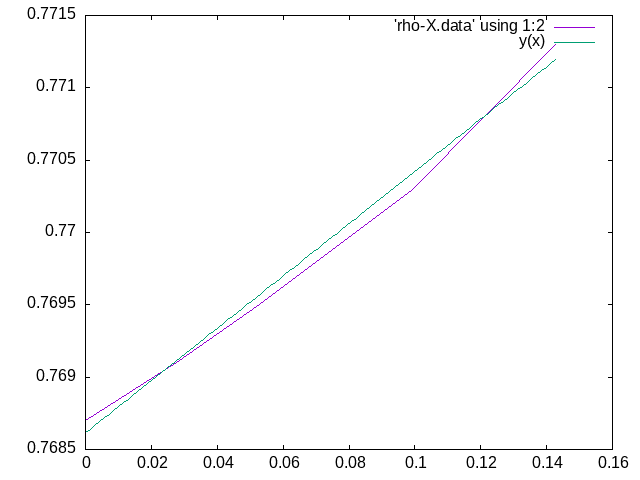
\includegraphics[width=.9\linewidth]{../data/rho-X.png}
\end{center}


\begin{verbatim}
iter      chisq       delta/lim  lambda   k             b            
   0 4.4675967090e-01   0.00e+00  7.09e-01    1.000000e+00   1.000000e+00
   1 1.5069310408e-02  -2.86e+06  7.09e-02    9.585995e-01   7.346859e-01
   2 8.9799960251e-04  -1.58e+06  7.09e-03    2.808739e-01   7.516539e-01
   3 4.9186716599e-08  -1.83e+09  7.09e-04    1.910146e-02   7.685483e-01
   4 3.5721637589e-08  -3.77e+04  7.09e-05    1.808388e-02   7.686141e-01
   5 3.5721637569e-08  -5.70e-05  7.09e-06    1.808384e-02   7.686141e-01
iter      chisq       delta/lim  lambda   k             b            

After 5 iterations the fit converged.
final sum of squares of residuals : 3.57216e-08
rel. change during last iteration : -5.69721e-10

degrees of freedom    (FIT_NDF)                        : 3
rms of residuals      (FIT_STDFIT) = sqrt(WSSR/ndf)    : 0.00010912
variance of residuals (reduced chisquare) = WSSR/ndf   : 1.19072e-08

Final set of parameters            Asymptotic Standard Error
=======================            ==========================
k               = 0.0180838        +/- 0.0009569    (5.292%)
b               = 0.768614         +/- 7.866e-05    (0.01023%)

correlation matrix of the fit parameters:
#                k      b      
k               1.000 
b              -0.784  1.000 

\end{verbatim}
\[
\rho=0.018084x+0.768614
\]

由于\(\beta\)=k/\(\rho\)\textsubscript{1}
\[
\beta=0.018084/0.7687=0.02353
\]
\section{根据溶液摩尔分数和折光率作图}
\label{sec:orgb39b221}
由于
\[
n=n_{1}(1+\gamma X)
\]
\begin{center}
\begin{tabular}{rr}
摩尔分数 & 折光率平均(nD)\\
\hline
0.00000 & 1.42087\\
0.02748 & 1.41957\\
0.05278 & 1.41867\\
0.09940 & 1.41710\\
0.14271 & 1.41573\\
\end{tabular}
\end{center}
\begin{center}
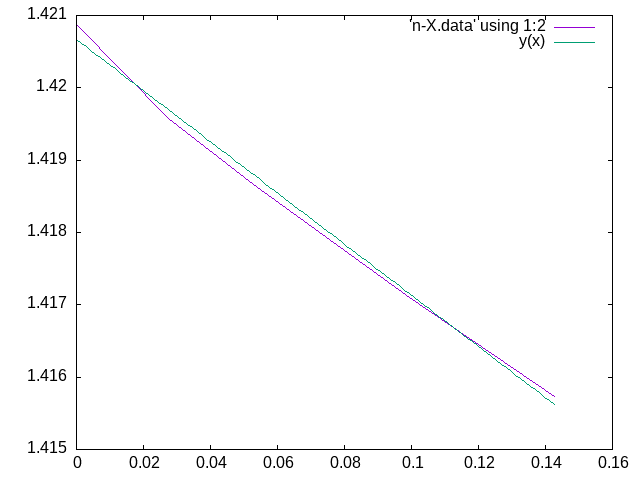
\includegraphics[width=.9\linewidth]{../data/n-X.png}
\end{center}
\begin{verbatim}
iter      chisq       delta/lim  lambda   k             b            
   0 6.4021482750e-01   0.00e+00  7.09e-01    1.000000e+00   1.000000e+00
   1 1.9033137369e-02  -3.26e+06  7.09e-02    9.941590e-01   1.321885e+00
   2 1.0844066593e-03  -1.66e+06  7.09e-03    2.533942e-01   1.401970e+00
   3 1.0490302753e-07  -1.03e+09  7.09e-04   -3.425735e-02   1.420597e+00
   4 8.8643557856e-08  -1.83e+04  7.09e-05   -3.537553e-02   1.420669e+00
   5 8.8643557831e-08  -2.77e-05  7.09e-06   -3.537558e-02   1.420669e+00
iter      chisq       delta/lim  lambda   k             b            

After 5 iterations the fit converged.
final sum of squares of residuals : 8.86436e-08
rel. change during last iteration : -2.77117e-10

degrees of freedom    (FIT_NDF)                        : 3
rms of residuals      (FIT_STDFIT) = sqrt(WSSR/ndf)    : 0.000171895
variance of residuals (reduced chisquare) = WSSR/ndf   : 2.95479e-08

Final set of parameters            Asymptotic Standard Error
=======================            ==========================
k               = -0.0353756       +/- 0.001507     (4.261%)
b               = 1.42067          +/- 0.0001239    (0.008723%)

correlation matrix of the fit parameters:
#                k      b      
k               1.000 
b              -0.784  1.000 

\end{verbatim}

\[
n=-0.03538X+1.42067
\]
由于\(\gamma\) =k/n\textsubscript{1}
\[
\gamma =-0.02490
\]

\section{根据溶液摩尔分数和介电常数作图}
\label{sec:org6a5e971}
算出 Co、Cd 和 \(\varepsilon\)\textsubscript{溶},由 \(\varepsilon\)\textsubscript{溶} = C\textsubscript{溶} / Co 算出  \(\varepsilon\)\textsubscript{溶},作 \(\varepsilon\)\textsubscript{溶}-X\textsubscript{2} 图,由 \(\alpha\) = 斜率 /\(\varepsilon\)\textsubscript{环}
 算出 \(\alpha\)。

联立以下三个式子:
\[
\varepsilon_{环}=C_{环}/Co=2.023-0.0016(t-20)
\]
\[
C_{环}'=C_{环}+Cd =5.90
\]
\[
C'o=Co+Cd=3.56
\]
解得:
\[
C_{o}=2.2874PF
\]
\[
C_{d}=1.2726PF
\]
根据公式:
\[
\varepsilon=\frac{C-C_{d}}{C_{o}}
\]
计算出介电常数,填入原始数据表
\begin{center}
\begin{tabular}{rr}
摩尔百分比 & 介电常数\\
\hline
0.00000 & 2.023\\
0.02748 & 2.068\\
0.05278 & 2.124\\
0.09940 & 2.256\\
0.14271 & 2.415\\
\end{tabular}
\end{center}

\begin{center}
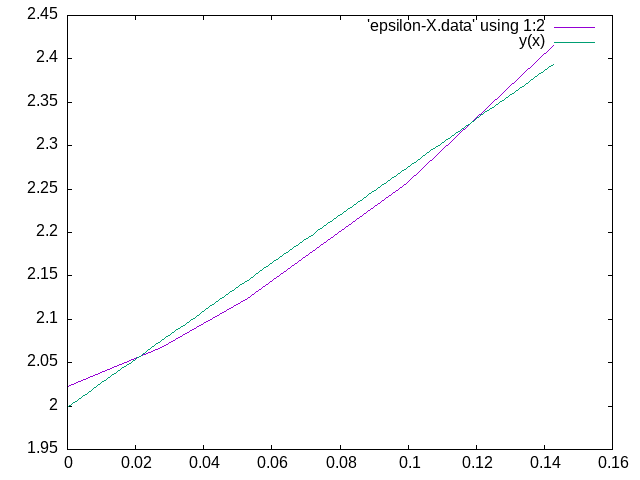
\includegraphics[width=.9\linewidth]{../data/epsilon-X.png}
\end{center}

\begin{verbatim}
function used for fitting: y(x)
	y(x)=k*x+b
fitted parameters initialized with current variable values

iter      chisq       delta/lim  lambda   k             b            
   0 6.2331685629e+00   0.00e+00  7.09e-01    1.000000e+00   1.000000e+00
   5 1.8396218585e-03  -3.37e-09  7.09e-06    2.765571e+00   1.998893e+00

After 5 iterations the fit converged.
final sum of squares of residuals : 0.00183962
rel. change during last iteration : -3.37115e-14

degrees of freedom    (FIT_NDF)                        : 3
rms of residuals      (FIT_STDFIT) = sqrt(WSSR/ndf)    : 0.024763
variance of residuals (reduced chisquare) = WSSR/ndf   : 0.000613207

Final set of parameters            Asymptotic Standard Error
=======================            ==========================
k               = 2.76557          +/- 0.2172       (7.852%)
b               = 1.99889          +/- 0.01785      (0.8931%)

correlation matrix of the fit parameters:
#                k      b      
k               1.000 
b              -0.784  1.000 

\end{verbatim}

\[
\varepsilon = 2.7658X+1.9989
\]
\[
\alpha=k/\varepsilon_{1}=2.7658/2.023=1.3672
\]
\section{计算P\textsuperscript{\infity}和R\textsuperscript{\infity}和固有偶极矩\(\mu\)}
\label{sec:org3779f48}
已经求得:
\begin{itemize}
\item \(\alpha\)=1.3672
\item \(\beta\)=0.02353
\item \(\gamma\)=-0.02490
\item \n\textsubscript{1}=1.42087
\item \(\varepsilon\)\textsubscript{1}=2.023
\item \(\rho\)\textsubscript{1}=0.7687
\item M\textsubscript{1}=84.16
\item M\textsubscript{2}=74.12
\item T=20\textsuperscript{o}C=293.15K

则有:
\end{itemize}
\[
P^{\infity}=P^{\infity}_{2}=\lim_{X_{2}\to 0}P_{2}=\frac{3\alpha\varepsilon_{1}}{(\varepsilon_{1}+2)^{2}}\cdot\frac{M_{1}}{\rho_{1}}+\frac{\varepsilon_{1}-1}{\varepsilon_{1}+2}\cdot\frac{M_{2}-\beta M_{1}}{\rho_{1}}  =79.99
\]
\[
R^{\infity}=R^{\infity}_{2}=\lim_{X_{2}\to 0}R_{2}=\frac{n_{1}^{2}-1}{n_{1}^{2}+2}\cdot\frac{M_{2}-\beta M_{1}}{\rho_{1}}+\frac{6n_{1}^{2}M_{1}r}{(n_{1}^{2}+2)^{2}\rho_{1}}=21.75
\]
\[
\mu=0.0128\sqrt{(79.99-21.75)*293.15}=1.67 Debye
\]
\end{document}
